\documentclass[12pt, a4paper]{report}
\usepackage[top=1.0in, bottom=1.0in, left=0.8in, right=0.8in]{geometry}

\setlength{\parskip}{\baselineskip}%
\setlength{\parindent}{0pt}%
\usepackage[]{graphicx}
\usepackage{enumitem}
\usepackage{amsmath}
\usepackage{relsize}
\usepackage{cprotect}
\usepackage{amsmath, amsfonts}
\usepackage{siunitx}
\usepackage{mathrsfs}
\usepackage{framed}
\usepackage{enumitem}
\usepackage{tikz}
\usepackage{circuitikz}
\usepackage{float}
\usepackage[english]{babel}
\usepackage{blindtext}

\newlist{notes}{enumerate}{1}
\setlist[notes]{label=\textbf{Note:} ,leftmargin=*}

\newlist{hints}{enumerate}{1}
\setlist[hints]{label=\textbf{Hint:} ,leftmargin=*}

\usepackage{xcolor}
\usepackage{color}
\definecolor{com1}{RGB}{125,125,125}
\definecolor{comment}{RGB}{140,115,115}
\definecolor{numbering}{rgb}{0.2,0.2,0.2}
\definecolor{key}{RGB}{0,0,180}
\definecolor{in}{RGB}{0,100,0}
\definecolor{out}{RGB}{100,30,30}
\definecolor{bg}{RGB}{245,245,245}
\definecolor{bgLight}{RGB}{250,250,250}
\definecolor{string}{RGB}{0,150,0}

\usepackage{hyperref}
\hypersetup{
    colorlinks=true,
    linkcolor=blue,
    filecolor=magenta,      
    urlcolor=blue,
}
\urlstyle{same}

\usepackage{listings}

\lstdefinestyle{py_code}{ %
    backgroundcolor=\color{bg},      % choose the background
    basicstyle=\ttfamily\small,		      % fonts
    breakatwhitespace=false,         % automatic breaks at whitespace ?
    breaklines=true,                 % sets automatic line breaking
    captionpos=b,                    % caption-position - bottom
    commentstyle=\itshape\color{comment},    % comment style
    extendedchars=true,              % use non-ASCII
    frame=single,	                   % single frame around the code
    keepspaces=true,                 % keeps spaces in text
    keywordstyle=\bfseries\color{key},% keyword style
    language=Python,                 	  % the language of the code
    morekeywords={Null},       % add more keywords to the set
    numbers=left,                    % line_numbers (none, left, right)
    numbersep=10pt,                  % line_no - code dist
    numberstyle=\footnotesize\color{numbering}, % line_no style
    rulecolor=\color{black},         % frame_color [!always set]
    showspaces=false,                % show spaces everywhere
    showstringspaces=false,          % 
    showtabs=false,                  % 
    stepnumber=1,                    % step b/w two line-no
    stringstyle=\color{string},     % string literal style
    tabsize=2,	                       % sets default tabsize to 2 spaces
    title=\lstname,                  % show the filename
    escapeinside={(*}{*)},			  % escape from style inside (* *)
    xleftmargin=\parindent,
    belowskip=-1.3 \baselineskip,
    aboveskip=1.0 \baselineskip,
    columns=fullflexible,
    xleftmargin=0.15in,
}
\lstnewenvironment{py_code}
{\lstset{style=py_code}}
{}

\lstdefinestyle{psudo}{ %
    backgroundcolor=\color{bgLight},   % choose the background
    basicstyle=\ttfamily\small,		      % fonts
    breakatwhitespace=false,         % automatic breaks at whitespace ?
    breaklines=true,                 % sets automatic line breaking
    captionpos=b,                    % caption-position - bottom
    commentstyle=\itshape\color{com1},          % comment style
    extendedchars=true,              % use non-ASCII
    keepspaces=true,                 % keeps spaces in text
    language=C,                 	  % the language of the code
    morekeywords={type,NULL, True, False},       % add more keywords to the set
    showspaces=false,                % show spaces everywhere
    showstringspaces=false,          % 
    showtabs=false,                  % 
    tabsize=2,	                       % sets default tabsize to 2 spaces
    title=\lstname,                  % show the filename
    escapeinside={(*}{*)},			  % escape from style inside (* *)
    belowskip=-1.8 \baselineskip,
    aboveskip=0.9 \baselineskip,
    columns=fullflexible,
    xleftmargin=0.2in,
    frame=tb,
    framexleftmargin=16pt,
    framextopmargin=6pt,
    framexbottommargin=6pt, 
    framerule=0pt,
}

\lstnewenvironment{psudo}
{\lstset{style=psudo}}
{}

\graphicspath{ ./ }


\title{\textbf{EE2703 : Applied Programming Lab \\ Final Exam 2019}} 
\author{Name of the students \\ Roll number} % Author name

\date{\today} % Date for the report

\begin{document}		
		
\maketitle % Insert the title, author and date
\section*{Q1}
 Input short summary of the question here which includes required  \textbf{formulas and facts and properties.} 
 
 \begin{equation}\label{eq:1}
 V_{n1}-V_{n2}=I_{n1,n2} R_{n1,n2}
 \end{equation}
 Multiple equations:
 \begin{align}
    f(x) &= x^{2-\alpha}\\
    g(x) &= \frac{1}{x}\\
    F(x) &= \int_{0}^{x} f(u)\,du\\
    f'(x) &= \frac{d}{dx}f(x)\\
    A    &= \begin{bmatrix}
            a_{1 1} & a_{1 0} \\
            a_{0 1} & a_{0 0}
           \end{bmatrix}\\
    \frac{\partial Q}{\partial t} &= \frac{\partial s}{\partial t}
 \end{align}
 To insert equation without numbering.
 \begin{equation*}
 V_{n1}-V_{n2}=L_{n1,n2} \frac{dI_{n1,n2}}{dt}
 \end{equation*}
 
 Here are some inline math: $ \alpha = \frac{\beta + \Phi (\phi) }{\Theta ( \theta )} $
 
 
 
 
 
 
\subsection*{Codes}
 To insert inline command you can use \texttt{print("Hello World")} \\
To type block of code manually use the following block
\begin{verbatim}	
    x = fun1(x1, x2, x3)
    z = fun2(z1, z2, z3)
    print('x = %d and z = %d' % (x,z))
\end{verbatim}
Python code:
\begin{py_code}
    x = fun1(x1, x2, x3)
    z = fun2(z1, z2, z3)
    print('x = %d and z = %d' % (x,z))
\end{py_code}
psudo code:
\begin{psudo}
This is a psudo code
sum = 0
for i in 0-10:
    sum += i
display sum
\end{psudo}

\subsection*{Results}
Include all the plots asked in the question here.
 \begin{figure}[H]
	\centering
	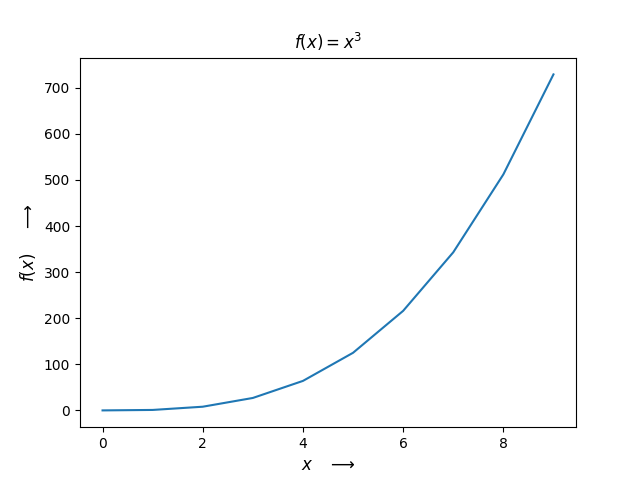
\includegraphics[scale=0.8]{Figure_1.png}  % Mention the image name within the curly braces. Image should be in the same folder as the tex file. 
	\caption{Sample image}
	\label{fig:sample}
\end{figure} 


\subsection*{Conclusions}
Figure~\ref{fig:sample} is the sample image  \\
Equation ~\ref{eq:1} is the sample equation 
   \begin{itemize}
  	\item One
  	\item Two
  \end{itemize}
  If you want to number them:
  \begin{enumerate}
      \item One 
      \item Two
  \end{enumerate}
% Repeat the above sections for the rest of the question. 

\end{document}



 